
\labday{Mercredi, 6 avril 2016}
\label{day:06-04-2016}

\experiment{Utiliser l'adversarial pour améliorer le correcteur}

\begin{figure}[H]
\centering
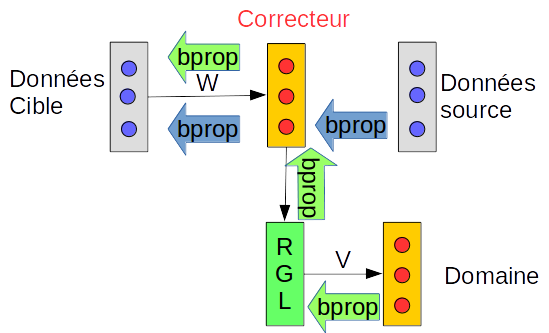
\includegraphics[width=0.45\linewidth]{fig/05-04-2016/Correcteur-Adversarial.png}
\caption{Correcteur adversarial}
\label{fig:correcteur_adversarial2}
\end{figure}

{\huge \textsc{Épic fail !}}

Non mais vraiment, ça marche pas du tout. Les résultats sont au mieux 
identiques (quand $\lambda_D\approx 0$) quelque soient les données que j'ai utilisées.


\experiment{Apprendre l'alignement}

Utiliser uniquement les classes pour déterminer l'alignement n'est pas suffisant.


%----------------------------------------------------------------------------------------
